
\subsection{Linux - Etcher}

Nach dem Download, muss man die erhaltene Datei "`2019-04-26-Raspjamming-full.img.7z"' entpacken.  Dies kann �ber den Browser und Dateimanager oder �ber die Konsole erfolgen.

\begin{console}
	wget --trust-server-names http://strohmayers.com/image/2019-04-26-Raspjamming-full.img.7z
	7z e 2019-04-26-Raspjamming-full.img.7z
	rm 2019-04-26-Raspjamming-full.img.7z
\end{console}

Das grafische Programm Etcher (Download auf \url{https://www.balena.io/etcher/}) kann zum �bertragen der Image-Datei verwendet werden. Es ist vor Allem f�r Anf�nger zu empfehlen, da beim Konsolenprogramm dd das Risiko besteht, dass Daten einer falschen Partition bzw. eines Laufwerks zerst�rt werden. Das Programm muss allerdings manuell installiert werden.     

\begin{console}
	wget https://github.com/balena-io/etcher/releases/download/v1.5.43/\
	balena-etcher-electron-1.5.43-linux-x64.zip
	unzip balena-etcher-electron-1.5.43-linux-x64.zip
	sudo mv balenaEtcher-1.5.43-x64.AppImage /usr/local/bin/etcher
	etcher &
\end{console}


%Nach dem Starten wird danach gefragt ob eine Verkn�pfung zum Programm erstellt werden soll. Dies sollte man mit "`Yes"' beantworten.\\ 
Mit der Schaltfl�che "`Select image"' kann man die Image-Datei "`2019-04-26-Raspjamming-full.img"' ausw�hlen. Ist nur ein m�gliches Ziel vorhanden, wird es bereits vorausgew�hlt, z.~B. die MicroSD-Karte im Karten-Slot (/dev/memcblk0) oder im USB-Adapter (/dev/sdb). Sind mehrere m�gliche Ziele vorhanden, wird die "`Select drive"' Schaltfl�che freigeschaltet. Dann kann ein Laufwerk manuell ausgew�hlt werden.

\begin{figure}[ht]
	\centering
	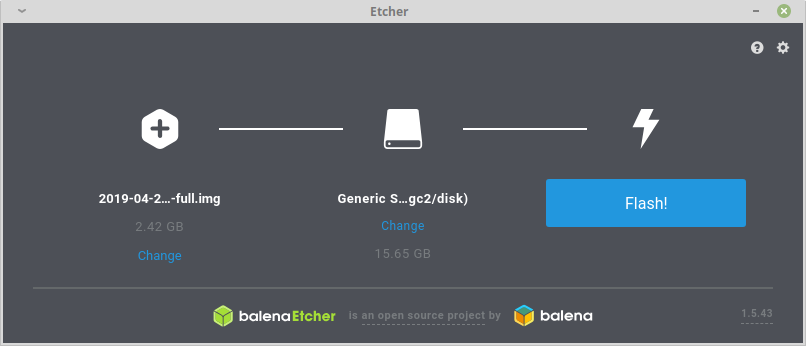
\includegraphics[scale=0.3]{images/Etcher.png}
	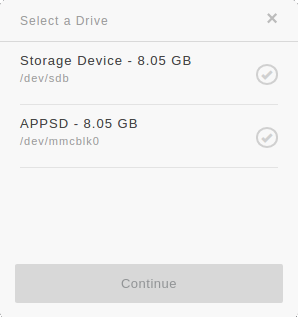
\includegraphics[scale=0.3]{images/Etcher_2.png}
	\label{Etcher}
\end{figure}


Wenn man noch etwas �ndern will, kann die entsprechende "`Change"' Schaltfl�che ausgew�hlt werden. Zum Schluss wird der Schreibvorgang mit der "`Flash!"' Schaltfl�che gestartet. M�glicherweise wird vom Programm allerdings noch das System-Passwort abgefragt.\\ 
Das Laufwerk bzw. die Partitionen werden nun aus dem System ausgeh�ngt und der Schreibvorgang gestartet. Der Fortschritt, die durchschnittliche �bertragungsrate und die Restlaufzeit werden w�hrend des Vorgangs angezeigt.
